\documentclass[11pt]{article}
\usepackage{certmachine}
%% generated by tools/paper-numbers/erdos290.js from certs/erdos290-tail-ext.json, certs/erdos290-tail-shard-*.json, legacy/research/challenges/erdos290/{kernel.js,tail-deltas.json,narrowing.json,theorem.js} and machine/erdos290/tail.js — do not edit (git eece01c1497a)
\newcommand{\RepoCommit}{eece01c1497a}
\newcommand{\CitedL}{60}
\newcommand{\CitedD}{120}
\newcommand{\HorizonL}{310}
\newcommand{\HorizonD}{620}
\newcommand{\ExtCount}{250}
\newcommand{\ExtFrom}{61}
\newcommand{\ExtTo}{310}
\newcommand{\ExtOpen}{0}
\newcommand{\ExtGenerated}{tools/run-erdos290-tail-ext.js + tail-shard merge @ git 325d9c1}
\newcommand{\ExtGit}{325d9c1}
\newcommand{\ExtCommitDate}{2026-08-31}
\newcommand{\NarrowGenerated}{2026-08-03}
\newcommand{\LegTailGenerated}{2026-08-03}
\newcommand{\ExtPrimes}{400}
\newcommand{\ExtB}{244}
\newcommand{\ExtESzero}{6}
\newcommand{\LegTailCount}{30}
\newcommand{\DeltaTopNum}{731}
\newcommand{\DeltaTopDen}{732}
\newcommand{\ShardCount}{6}
\newcommand{\ShardTotal}{190}
\newcommand{\ShardFrom}{121}
\newcommand{\ShardTo}{310}
\newcommand{\SerialCount}{60}
\newcommand{\SerialTo}{120}
\newcommand{\TimeLowSecs}{116}
\newcommand{\TimeLowL}{91}
\newcommand{\TimeHighSecs}{212}
\newcommand{\TimeHighL}{105}
\newcommand{\TimeExponent}{4.2}
\newcommand{\ExcRows}{1 & 8 & 4 & \texttt{galois8.js} & 0.390625000000 & $<10^{-2}$ \\
2 & 24 & 12 & \texttt{galois-exceptions.js} & 0.393469340286 & $<10^{-12}$ \\
3 & 48 & 24 & \texttt{galois-exceptions.js} & 0.393469340287 & $<10^{-31}$ \\
4 & 80 & 40 & \texttt{tail-deltas.json} & 0.393469340287 & $<10^{-59}$ \\
5 & 120 & 60 & \texttt{tail-deltas.json} & 0.393469340287 & $<10^{-99}$ \\
6 & 168 & 84 & \texttt{tail-ext.json} & 0.393469340287 & $<10^{-151}$ \\
7 & 224 & 112 & \texttt{tail-ext.json} & 0.393469340287 & $<10^{-216}$ \\
8 & 288 & 144 & \texttt{tail-ext.json} & 0.393469340287 & $<10^{-293}$ \\
9 & 360 & 180 & \texttt{tail-ext.json} & 0.393469340287 & $<10^{-383}$ \\
10 & 440 & 220 & \texttt{tail-ext.json} & 0.393469340287 & $<10^{-487}$ \\
11 & 528 & 264 & \texttt{tail-ext.json} & 0.393469340287 & $<10^{-605}$ \\}
\newcommand{\ExcCount}{11}
\newcommand{\ExcMaxK}{11}
\newcommand{\ExcMaxD}{528}
\newcommand{\ExcExtCount}{6}
\newcommand{\ExcExtList}{168, 224, 288, 360, 440 and 528}
\newcommand{\ExcCitedList}{8, 24, 48, 80 and 120}
\newcommand{\ExcPaperList}{8, 24 and 48}
\newcommand{\DiscRows}{2 & 1 & 3 & 1 & 12 & not a square \\
4 & 2 & 5 & 145 & 6{,}728{,}000 & not a square \\
6 & 3 & 7 & 12{,}510{,}288 & 2{,}524{,}149{,}828{,}635{,}000{,}832 & not a square \\
8 & 4 & 9 $=3^2$ & 2{,}303{,}072{,}868{,}513{,}024 & 37 digits & square \\}
\newcommand{\TheoremSecs}{14}
\newcommand{\TheoremChecks}{13}
\newcommand{\TheoremFalsifiers}{3}
\newcommand{\TheoremDegrees}{40}
\newcommand{\TheoremMaxD}{80}
\newcommand{\TheoremLawMaxD}{624}
\newcommand{\WitnessCount}{27}
\newcommand{\WitnessMaxP}{1087}
\newcommand{\SensOne}{4}
\newcommand{\SensTwo}{5}
\newcommand{\SensThree}{6}
\newcommand{\KernelChecks}{17}
\newcommand{\KernelFalsifiers}{3}
\newcommand{\PatternDigits}{45{,}336}
\newcommand{\PatternControls}{24}
\newcommand{\PatternFrom}{122}
\newcommand{\PatternTo}{170}
\newcommand{\PatternSecs}{23}
\newcommand{\LeanPass}{6}
\newcommand{\LeanMaxL}{12}
\newcommand{\CLo}{0.830416407911}
\newcommand{\CHi}{0.831220912621}
\newcommand{\CWidth}{$8.045\times10^{-4}$}
\newcommand{\CWidthSixty}{$4.115\times10^{-3}$}
\newcommand{\CWidthThirty}{$8.130\times10^{-3}$}
\newcommand{\WidthGainPct}{80\%}
\newcommand{\WidthFactorSixty}{5.1}
\newcommand{\InvLo}{0.546083759260}
\newcommand{\InvHi}{0.546323774021}
\newcommand{\InvAgreed}{3}
\newcommand{\InvSixtyAgreed}{2}
\newcommand{\InvThirtyAgreed}{2}
\newcommand{\InvPrefix}{0.546}
\newcommand{\InvSixtyPrefix}{0.54}
\newcommand{\InvSixtyLo}{0.545485611000}
\newcommand{\InvSixtyHi}{0.546712849449}
\newcommand{\CSixtyLo}{0.829113767875}
\newcommand{\CSixtyHi}{0.833228924528}
\newcommand{\CThirtyLo}{0.827534229497}
\newcommand{\CThirtyHi}{0.835663773592}
\newcommand{\InvThirtyLo}{0.544762071565}
\newcommand{\InvThirtyHi}{0.547185373527}
\newcommand{\InvWidth}{$2.400\times10^{-4}$}
\newcommand{\InvHiFour}{0.5464}
\newcommand{\InvLoThree}{0.546}
\newcommand{\TwoCHi}{0.602107563430}
\newcommand{\TwoCSixtyHi}{0.603053548708}
\newcommand{\VDLo}{0.54}
\newcommand{\VDHi}{0.61}
\newcommand{\VDCLo}{0.82}
\newcommand{\VDCHi}{0.85}
\newcommand{\VDWidth}{0.07}
\newcommand{\NewWidth}{0.0560}
\newcommand{\VDInvLo}{0.5405}
\newcommand{\VDInvHi}{0.5495}
\newcommand{\VDTwoCHi}{0.6098}
\newcommand{\LogTwoLo}{0.693147180559945}
\newcommand{\LogTwoHi}{0.693147180559946}
\newcommand{\LogTwoShare}{83\%}
\newcommand{\EvenPinned}{0.137269227351}
\newcommand{\TailLo}{0.000804504708}
\newcommand{\TailHi}{0.000804504709}
\newcommand{\TailWeight}{$8.045\times10^{-4}$}
\newcommand{\TailApprox}{$8.065\times10^{-4}$}
\newcommand{\HorizonRows}{30 & 60 & 0.827534229497 & 0.835663773592 & $8.13\times10^{-3}$ & 0.544762071565 & 0.547185373527 & 2 \\
60 & 120 & 0.829113767875 & 0.833228924528 & $4.12\times10^{-3}$ & 0.545485611000 & 0.546712849449 & 2 \\
90 & 180 & 0.829649026497 & 0.832403826529 & $2.75\times10^{-3}$ & 0.545731233215 & 0.546552910158 & 2 \\
120 & 240 & 0.829918323025 & 0.831988707526 & $2.07\times10^{-3}$ & 0.545854893041 & 0.546472477716 & 2 \\
190 & 380 & 0.830217269525 & 0.831527883265 & $1.31\times10^{-3}$ & 0.545992233663 & 0.546383217256 & 2 \\
250 & 500 & 0.830340663775 & 0.831337671758 & $9.97\times10^{-4}$ & 0.546048943033 & 0.546346382284 & 3 \\
310 & 620 & 0.830416407911 & 0.831220912621 & $8.05\times10^{-4}$ & 0.546083759260 & 0.546323774021 & 3 \\}
\newcommand{\ThirdDigitL}{197}
\newcommand{\ThirdDigitD}{394}
\newcommand{\ThirdDigitLo}{0.546000622219}
\newcommand{\ThirdDigitHi}{0.546377767763}
\newcommand{\ThirdDigitPrevLo}{0.545999460383}
\newcommand{\ThirdDigitPrevHi}{0.546378522515}
\newcommand{\CondDigits}{34}
\newcommand{\CondLo}{0.8307329558487356638503727480334797}
\newcommand{\CondHi}{0.8307329558487356638503727480334798}
\newcommand{\CondInv}{0.546229310400104587}
\newcommand{\CondFirstL}{31}
\newcommand{\CondFirstD}{62}
\newcommand{\CondAllowFirst}{$1.45\times10^{-47}$}
\newcommand{\CondCap}{46}
\newcommand{\CStarDigits}{110}
\newcommand{\CZeroDigits}{110}
\newcommand{\PrecCalib}{43}
\newcommand{\PrecCutoffA}{510}
\newcommand{\PrecCutoffB}{570}
\newcommand{\CStarForty}{0.8307329558487356638503727480334797472934}
\newcommand{\CZeroForty}{0.5462293104001045874126605854383631427348}
\newcommand{\CZeroFull}{0.5462293104\,0010458741\,2660585438\,3631427348\,3317015360\,2571994177\,1294105433\,3303218493\,6590239418\,1630751977\,3773368722}
\newcommand{\CStarFull}{0.8307329558\,4873566385\,0372748033\,4797472934\,3800478380\,4612152517\,2321583212\,5501966589\,9656233483\,2364655190\,1616522095}
\newcommand{\CZeroFullA}{5462293104\,0010458741\,2660585438\,3631427348\,3317015360\,2571994177}
\newcommand{\CZeroFullB}{1294105433\,3303218493\,6590239418\,1630751977\,3773368722}
\newcommand{\CStarFullA}{8307329558\,4873566385\,0372748033\,4797472934\,3800478380\,4612152517}
\newcommand{\CStarFullB}{2321583212\,5501966589\,9656233483\,2364655190\,1616522095}
\newcommand{\BfileTerms}{110}
\newcommand{\FailD}{622}
\newcommand{\FailC}{$2.58\times10^{-6}$}
\newcommand{\InvDeriv}{0.2985}
\newcommand{\FailInv}{$7.70\times10^{-7}$}
\newcommand{\CellLo}{0.5462}
\newcommand{\CellHi}{0.5463}
\newcommand{\WindowA}{0.0991}
\newcommand{\WindowB}{0.5155}
\newcommand{\DeltaLimit}{0.3934693}
\newcommand{\WindowMarginHi}{0.1221}
\newcommand{\WindowMarginLo}{0.2944}
\newcommand{\FourthL}{1{,}543}
\newcommand{\FourthD}{3{,}086}
\newcommand{\FourthWidth}{$1.62\times10^{-4}$}
\newcommand{\FourthCost}{614}


\DeclareMathOperator{\disc}{disc}
\DeclareMathOperator{\Gal}{Gal}
\DeclareMathOperator{\lead}{lead}
\DeclareMathOperator{\Res}{Res}
\DeclareMathOperator{\wt}{wt}
\newcommand{\lia}{\liminf_{a\to\infty}\frac{b(a)-a}{\log a}}
\renewcommand{\topfraction}{0.9}\renewcommand{\bottomfraction}{0.9}\renewcommand{\textfraction}{0.08}\renewcommand{\floatpagefraction}{0.85}
\newcommand{\Sl}{S_l^{+}}

\title{Erd\H{o}s problem 290: the $4k(k+1)$ square-discriminant law as exact integer identities, and a certified bracket for the Galois-density constant behind both endpoints of van Doorn's Theorem~8}
\author{\cmauthor}
\date{October 2026 --- draft v0.1 for review; every number interpolated from the record; machine-derived, not peer-reviewed; author list to be agreed}

\begin{document}
\maketitle

\begin{abstract}
For a positive integer $a$ let $b(a)$ be the least $b>a$ at which the denominator of $\frac1a+\dots+\frac1b$, in lowest terms, drops below that of $\frac1a+\dots+\frac1{b-1}$ (Erd\H{o}s problem 290). Van Doorn proved $0.54<\lia<0.61$, the two constants being $1/(1+c)$ and $1/(2c)$ to two decimals, where $c=\sum_{d\ge1}\delta(f_d)/(d(d+1))$, $\delta(f_d)$ is the density of primes modulo which the derivative $f_d$ of $x(x-1)\cdots(x-d)$ has a root, and $0.82<c<0.85$ comes from the Galois groups of $f_d$ for even $d\le60$: the signed symmetric group $\Sl$ except at $d=8,24,48$. We prove that for even $d=2l$, $\disc f_d=(d+1)(2^l\,l!\,\disc h_l)^2$ with $f_d(x+l)=h_l(x^2)$, so $\disc f_d$ is a perfect square exactly at $d=4k(k+1)$, the only even degrees at which the group can lie in the alternating group. We decide the density at every even $d\le\HorizonD$ by a five-candidate structural squeeze in exact arithmetic ($\Sl$ everywhere except the \ExcCount{} degrees $4k(k+1)\le\ExcMaxD$, where the group has index two) and, charging every undecided degree the whole interval $[0,1]$, obtain the certified bracket $c\in[\CLo,\CHi]$, $1/(1+c)\in[\InvLo,\InvHi]$: three decimals of the lower constant where the published statement had two, and $1/(2c)\le\TwoCHi$ against $0.61$. Van Doorn's note of 31 August 2026 proves that the liminf equals $1/(1+c)$, so the bracket is the certified value of the liminf itself, $\InvPrefix\ldots$, with no assumption about the tail (van Doorn's Lemma~32 Magma computation, even $d\le60$, taken as given); under one stated assumption on the groups past the horizon the expansion continues to \CStarDigits{} digits, and we say which digits are theorem digits and which only extend a decimal expansion. Every number is interpolated from a public record re-run at every build.
\end{abstract}

\section{Introduction}

Erd\H{o}s and Graham asked \cite[p.~34]{EG80}, and the problem page records \cite{EP290}: for $a\ge1$, must there be some $b>a$ such that, writing $\sum_{a\le n\le b}\frac1n=\frac{r_1}{s_1}$ and $\sum_{a\le n\le b+1}\frac1n=\frac{r_2}{s_2}$ in lowest terms, $s_2<s_1$; and if so, how does the least such $b=b(a)$ grow with $a$?\footnote{Van Doorn's $b(a)$ \cite{vD24,vD26} is the least $b>a$ with $v_{a,b}<v_{a,b-1}$, one more than the page's $b$; the liminf below is the same for both.} Van Doorn \cite{vD24} answered the first question affirmatively, with $b(a)\le4.374(a-1)$ for $a\ge6$, and for the lower order of growth proved (Theorem~8 there)
\begin{equation}\label{eq:thm8}
\VDLo<\lia<\VDHi .
\end{equation}
The proof of \eqref{eq:thm8} is three lemmas. With $f_d(x)=\sum_{i=0}^d\prod_{j\ne i}(x-j)$, the derivative of $\prod_{j=0}^d(x-j)$, let $\delta(f_d)$ be the density of primes $p$ for which $f_d(x)\equiv0\pmod p$ is solvable, and
\begin{equation}\label{eq:c}
c=\sum_{d\ge1}\frac{\delta(f_d)}{d(d+1)} .
\end{equation}
Lemma~31 of \cite{vD24} gives $\lia\ge\frac1{1+c}$, Lemma~30 gives $\lia\le\frac1{2c}$, and Lemma~32 gives $\VDCLo<c<\VDCHi$, ``from which $\frac1{2c}<\VDHi$ and $\frac1{1+c}>\VDLo$ follow by computation''. Both published constants are therefore two-decimal roundings of the same quantity read two ways. The proof of Lemma~32 is a computation: PARI finds $f_d$ irreducible for all even $d\le500$, Magma finds the Galois group $G_d$ isomorphic to the signed symmetric (hyperoctahedral) group $\Sl$, $l=d/2$, for all even $d\le60$ except $d=\ExcPaperList$; the odd degrees contribute exactly $\log2$, the even $d\le60$ off the exceptional set contribute about $0.1281$ under $\Sl$, and everything else is charged $\delta\le1$.

On 28 November 2025 van Doorn opened a help-wanted issue \cite{Issue164} asking for a computation of $c_0=1/(1+c)$, there bracketed as $0.54<c_0<0.55$, precise enough for an entry in the OEIS, and naming as the work the Galois groups $G_d$ at even $d$ and the derangement counts in the relevant subgroups of $\Sl$. This paper is the written form of the answer, in four parts.

\begin{enumerate}
\item A theorem (Section~\ref{sec:law}): for even $d=2l$, $\disc f_d=(d+1)(2^l\,l!\,\disc h_l)^2$, so $\disc f_d$ is a square exactly at $d=4k(k+1)$ (OEIS A033996 \cite{OEIS}), the only even degrees at which $G_d$ can lie in $A_{2l}$; $\{8,24,48\}$ is exactly the set of them below $60$. Each line of the five-line proof is also checked as an exact integer identity, with planted falsifiers that must fail.
\item A decided record (Section~\ref{sec:squeeze}): $\delta(f_d)$ as an exact rational at every even $d\le\HorizonD$, by a structural squeeze over five candidate groups: $\Sl$ everywhere except the \ExcCount{} degrees $4k(k+1)\le\ExcMaxD$, where the group is the even-weight subgroup of index two.
\item A certified bracket (Section~\ref{sec:bracket}): with every undecided degree charged $[0,1]$, $c\in[\CLo,\CHi]$ and $1/(1+c)\in[\InvLo,\InvHi]$, which moves both endpoints of \eqref{eq:thm8} (Section~\ref{sec:thm8}).
\item The day the bracket reached three decimals, van Doorn posted a note \cite{vD26} proving $\lia=\frac1{1+c}$ exactly; the upper endpoint is retired and the bracket becomes the certified value of the liminf, $\InvPrefix\ldots$, with no assumption about the tail and the Lemma~32 group computation taken as given (Table~\ref{tab:prov}). Under one stated assumption on the groups past the horizon the expansion continues to \CStarDigits{} digits (Section~\ref{sec:cond}); we separate the digits that sharpen a theorem from those that only extend a decimal expansion.
\end{enumerate}

Nothing in the arithmetic is new. What we offer as the contribution, beyond the theorem, is the decision grammar and the record: every even degree returns either a verdict with its witness (the certificates and the one surviving group) or a refusal that is costed (the degree keeps the whole interval $[0,1]$, and the bracket says what that ignorance costs); the bracket is monotone in the horizon by construction; and the whole chain is re-run from the public record at every build of the report page \cite{Report}, with falsifiers that must fire. A number the record does not hold cannot appear on the page or here.

\paragraph{Words.} A quantity is \emph{certified} when it is an exact rational computed from the record, or an interval whose endpoints are exact rationals rounded outward to the printed digits, and the program producing it is re-run with its controls at every build; a verdict about a group is \emph{decided}; Theorem~\ref{thm:law} is \emph{proved}; results of \cite{vD24} that we recompute are \emph{re-decided}.

\section{The constant and the polynomials}\label{sec:setup}

$f_d$ has degree $d$, leading coefficient $d+1$, and $d$ distinct real roots (Rolle, since $\prod_{j=0}^d(x-j)$ has $d+1$ distinct real roots). The density $\delta(f_d)$ exists by Chebotarev. Four facts from \cite{vD24} fix the shape of \eqref{eq:c}.

\begin{itemize}
\item (Lemma~37) $f_d(d-x)=(-1)^df_d(x)$, so $f_d(x+\frac d2)$ is odd for odd $d$ and even for even $d$. For odd $d$, $\frac d2$ is a rational root, hence $\delta(f_d)=1$ and the odd degrees contribute $\sum_{k\ge0}\bigl(\frac1{2k+1}-\frac1{2k+2}\bigr)=\log2$ to $c$ exactly: this is \LogTwoShare{} of the constant.
\item (Lemma~38) If $f_d$ is irreducible, $\delta(f_d)$ is the proportion of elements of $G_d=\Gal(f_d)$, acting on the roots, that are not derangements (Frobenius).
\item (Lemma~39) For even $d=2l$ write $f_d(x+l)=h_l(x^2)$ with $h_l$ of degree $l$. The roots of $f_d$ pair as $l\pm\rho_i$, and $G_d$ embeds in $\Sl=C_2^l\rtimes S_l$, the group of signed permutations of the $l$ pairs, of order $2^l\,l!$.
\item (Lemma~40) The non-derangement fraction of $\Sl$ itself is
\begin{equation}\label{eq:hyp}
\delta_{\mathrm{hyp}}(l)=1-\sum_{i=0}^{l}\frac{(-1)^i}{2^i\,i!}\;\longrightarrow\;1-e^{-1/2}=\DeltaLimit\ldots
\end{equation}
\end{itemize}
Write an element of $\Sl$ as $(v,\sigma)$ with $v\in\mathbb F_2^l$ the sign vector and $\sigma\in S_l$, and let $E=\{(v,\sigma):\wt v\equiv0\pmod2\}$ be the even-weight subgroup, of index two. A signed cycle of $\sigma$ is negative when the weight of $v$ on it is odd, and a negative $k$-cycle is a $2k$-cycle on the $2k$ roots it moves while a positive one is two $k$-cycles; so $(v,\sigma)$ is an even permutation of the $2l$ roots exactly when $\wt v$ is even, that is $E=\Sl\cap A_{2l}$. Its non-derangement fraction differs from \eqref{eq:hyp} at one element only: given $\sigma$ with $f<l$ fixed points, exactly half of the sign vectors that make every fixed point negative have even weight, so the conditional probability of a derangement is $2^{-f}$ in both groups; at $\sigma=\mathrm{id}$ it is $2^{-l}$ in $\Sl$ and, for even $l$, $2^{-(l-1)}$ in $E$. Hence for even $l$
\begin{equation}\label{eq:index2}
\delta(E)=\delta_{\mathrm{hyp}}(l)-\frac1{2^l\,l!}.
\end{equation}
So $c=\log2+\sum_{l\ge1}\delta(f_{2l})\,w_l$ with $w_l=\frac1{2l(2l+1)}$, and $\sum_{l\ge1}w_l=1-\log2$ by telescoping. The whole difficulty is the even degrees: which group, and therefore which rational, each one carries.

\section{The square-discriminant law}\label{sec:law}

For a polynomial $g$ of degree $n$ with leading coefficient $a$ and roots $s_1,\dots,s_n$, $\disc g=a^{2n-2}\prod_{i<j}(s_i-s_j)^2$.

\begin{lemma}[composition with $x^2$]\label{lem:comp}
Let $h\in\Z[x]$ have degree $l\ge1$, leading coefficient $a$ and $h(0)\ne0$. Then
\[
\disc h(x^2)=(-1)^l\,2^{2l}\,a\,h(0)\,(\disc h)^2 .
\]
\end{lemma}
\begin{proof}
Let $r_1,\dots,r_l$ be the roots of $h$, so $\prod_ir_i=(-1)^lh(0)/a\ne0$, and $g=h(x^2)$ has degree $2l$, leading coefficient $a$ and roots $\pm\sqrt{r_i}$. The pair $\{\sqrt{r_i},-\sqrt{r_i}\}$ contributes $(2\sqrt{r_i})^2=4r_i$; for $i<j$ the four differences $\pm\sqrt{r_i}\pm\sqrt{r_j}$ multiply to $(r_i-r_j)^2$, so their squares contribute $(r_i-r_j)^4$. Hence
$\disc g=a^{4l-2}\cdot4^l\prod_ir_i\cdot\prod_{i<j}(r_i-r_j)^4
=a^{4l-2}\cdot4^l\,\frac{(-1)^lh(0)}a\cdot\frac{(\disc h)^2}{a^{4l-4}}$,
which is the claim.
\end{proof}

This is the special case $g=x^2$ of the discriminant of a composition, written down in general for non-monic polynomials by Cullinan \cite{Cullinan} ($\disc f\circ g=(-1)^{\epsilon\delta(3\epsilon\delta-2\delta-1)/2}\,\ell(f)^{\delta-1}\ell(g)^{\epsilon(\epsilon\delta-1)}(\disc f)^\delta\Res(f\circ g,g')$, under $\Res(f,g)\ne0$); its hypotheses hold here since $\Res(h,x^2)=h(0)^2\ne0$. The two-line proof above keeps the paper self-contained. The leading coefficient is the whole point: in monic form the criterion below would read $(-1)^lh(0)=(l!)^2$, always a square.

\begin{theorem}\label{thm:law}
Let $d=2l$ be even and let $h_l$ be the polynomial with $f_d(x+l)=h_l(x^2)$. Then
\begin{enumerate}
\item[(a)] $h_l(0)=(-1)^l(l!)^2$, $\lead h_l=d+1$, and $\disc h_l\ne0$;
\item[(b)] $\disc f_d=(d+1)\bigl(2^l\,l!\,\disc h_l\bigr)^2$;
\item[(c)] $\disc f_d$ is a perfect square if and only if $d+1$ is, that is, if and only if $d=4k(k+1)$ for some integer $k\ge1$.
\end{enumerate}
\end{theorem}
\begin{proof}
$h_l$ exists by Lemma~37 of \cite{vD24}. (a) $f_d(l)=\sum_i\prod_{j\ne i}(l-j)$, and every summand but $i=l$ carries the factor $(l-l)$, so $f_d(l)=\prod_{j\ne l}(l-j)=l!\cdot(-1)^ll!$. The leading coefficient of $h_l$ is that of $f_d$, which is $d+1$ as the derivative of a monic polynomial of degree $d+1$. The $d$ roots of $f_d$ are real and distinct and none equals $l$ (as $f_d(l)\ne0$), so $f_d(x+l)$ has $2l$ distinct non-zero real roots $\pm\rho_1,\dots,\pm\rho_l$ and $h_l$ has the $l$ distinct roots $\rho_i^2$. (b) $\disc f_d=\disc f_d(x+l)$, and Lemma~\ref{lem:comp} with $a=d+1$ and $h(0)=(-1)^l(l!)^2$ gives $(-1)^l2^{2l}(d+1)(-1)^l(l!)^2(\disc h_l)^2$. (c) By (b) and (a), $\disc f_d=(d+1)B^2$ with $B$ a non-zero integer, so it is a square exactly when $d+1$ is; $d+1$ is odd, so $d+1=(2k+1)^2$ and $d=4k(k+1)$.
\end{proof}

\begin{corollary}\label{cor:law}
For even $d=2l$, $G_d\subseteq A_{2l}$, equivalently $G_d\subseteq E$, if and only if $d=4k(k+1)$. In particular the three exceptional degrees of Lemma~32 of \cite{vD24} are exactly the $4k(k+1)<60$, and no other even degree can have its group inside the even-weight subgroup.
\end{corollary}
\begin{proof}
$G_d\subseteq A_{2l}$ iff $\disc f_d$ is a square; $E=\Sl\cap A_{2l}$ by Section~\ref{sec:setup}.
\end{proof}

\begin{remark}
The corollary is a containment statement. Whether $G_d$ actually drops into $E$ at a given $4k(k+1)$, and whether some degree drops to a proper subgroup of $\Sl$ not contained in $A_{2l}$, which a non-square discriminant does not forbid, are per-degree questions; Section~\ref{sec:squeeze} answers them through $d=\HorizonD$ and nowhere else. Odd degrees are outside the statement and must be: there $\frac d2$ is a rational root, and $\disc f_1=1$ is a square.
\end{remark}

\paragraph{The identities, checked.} The program \texttt{theorem.js} of the record \cite{Report} checks every line of the proof as an exact integer identity, in BigInt arithmetic with no library: (a) at every even $d\le\TheoremMaxD$ (\TheoremDegrees{} degrees); Lemma~\ref{lem:comp} on its own, on seven random polynomials, monic and not, and on $h_4,h_{12},h_{24}$, so that the leading factor cannot pass by a coincidence of the family; (b) exactly at every even $d\le\TheoremMaxD$; $\disc h_l\ne0$ at every swept degree; the equivalence (c) at every swept degree; and the arithmetic of the conclusion, $\{\text{even }d\le\TheoremLawMaxD:d+1\text{ square}\}=\{4k(k+1)\}$. Discriminants are computed by Chinese remaindering over word-size primes under a Hadamard bound and, independently, by a Sylvester matrix with Bareiss elimination; the two agree on $f_d$ and $h_l$ for even $d\le20$. Three planted falsifiers must break the identity: $\disc h_l+1$, $d+1\to d+2$, and indexing the product from $1$ instead of $0$ (degree $d-1$, $f(x+\frac d2)$ not even, discriminant not a square at $d=8$), a draft's error kept as a control. The run reports \TheoremChecks{} checks passed, the \TheoremFalsifiers{} planted falsifiers among them, in \TheoremSecs{} s on the machine that built this document. A second program, \texttt{pattern-check.js}, predates the proof: written while the law was a five-point conjecture, it computed $\disc f_{168}$ exactly (\PatternDigits{} decimal digits, \PatternSecs{} s) and found it a perfect square, while certifying every other even degree in $\PatternFrom..\PatternTo$ non-square by a quadratic non-residue witness (\PatternControls{} controls). It is kept as the blind $k=6$ confirmation, not as the evidence the law rests on. (The integer sequences $\disc f_d$ and $\disc h_l$ are, to our knowledge, not in the OEIS.)



\begin{remark}[on the first write-up]
The comment of 4 August 2026 on \cite{Issue164} credited the composition step to a 2020 paper on doubly even octic polynomials, in monic form, and presented the non-monic factor as the new step. On reading, that paper carries no general composition law; the general non-monic law is Cullinan's note \cite{Cullinan}, which the report page cites, and the correction was posted in the follow-up of 31 August 2026. The characterisation (c) we have not found anywhere: \cite{vD24} contains no discriminant, and A033996 \cite{OEIS} carries no comment relating it to polynomials or Galois groups.
\end{remark}

\section{Deciding the density at each even degree}\label{sec:squeeze}

Enumerating subgroups of $\Sl$ is possible at $l=4$ (the program \texttt{galois8.js} enumerates all subgroups of $S_4^+$ by closure and keeps those that are transitive, contain every observed cycle type and lie in $A_8$ exactly when the discriminant is a square; every survivor has the same non-derangement fraction, $\delta(f_8)=75/192=25/64$) and hopeless beyond. The instrument used for every other degree, \texttt{galois-exceptions.js} of the record, uses structure instead of enumeration.

\paragraph{Five candidates.} Let $G=G_d\le\Sl$, $K=G\cap C_2^l$ its sign kernel, and $\pi(G)\le S_l$ its image, which is $\Gal(h_l)$ acting on the $\rho_i^2$. Three classical facts:
\begin{itemize}
\item[(K)] $K$ is a $\pi(G)$-submodule of $\mathbb F_2^l$. When $\pi(G)\supseteq A_l$ the only submodules are $0$, $\langle(1,\dots,1)\rangle$, the even-weight module and $\mathbb F_2^l$; a certified element of $K$ of even weight $w$ with $0<w<l$ forces $K$ to contain the even-weight module, and an odd $w$ forces $K=\mathbb F_2^l$.
\item[($\pi$)] If $h_l$ is irreducible, $\pi(G)$ is transitive. A transitive group containing a $p$-cycle with $p$ prime and $p>l/2$ is primitive, and a primitive group of degree $l$ containing a $p$-cycle with $p\le l-3$ contains $A_l$ (Jordan's theorem, see \cite{Wielandt}). $\disc h_l$ is a square iff $\pi(G)\subseteq A_l$.
\item[($\pm$)] $G\subseteq A_{2l}$ iff $\disc f_d$ is a square iff every element of $G$ has even weight (Section~\ref{sec:setup}).
\end{itemize}
With $K\supseteq$ even-weight and $\pi(G)\supseteq A_l$ certified, exactly five groups remain: a full kernel lifts uniquely ($B=\Sl$, $FA=C_2^l\rtimes A_l$); an even-weight kernel leaves a homomorphism $\pi(G)\to C_2$ choosing the weight parity per $\sigma$, trivial or $\operatorname{sgn}$ on $S_l$ ($ES0=\{\wt v\equiv0\}$, $ESs=\{\wt v\equiv\operatorname{sgn}\sigma\}$), only trivial on $A_l$ ($EA0$). Each has an exact non-derangement fraction over the conjugacy classes of $S_l$.

\paragraph{The data.} For each prime $p$ not dividing $\disc f_d\cdot\disc h_l\cdot(d+1)$, the distinct-degree factorisation of $f_d$ and of $h_l$ modulo $p$ gives, by Dedekind's theorem \cite[Ch.~13]{Cox}, the cycle type of a Frobenius element on the $2l$ roots and of its projection on the $l$ pairs; the numbers of negative and positive cycles of each length are the unique solution of $n_m=2\,\mathrm{pos}_m+\mathrm{neg}_{m/2}$, $\mathrm{pos}_k+\mathrm{neg}_k=a_k$. Raising the element to the order of its projection lands in $K$, with weight $\sum k\cdot\mathrm{neg}_k$ over the cycle lengths $k$ whose cofactor in that order is odd. The certificates: $f_d$ irreducible over $\Q$ (no degree $1\le k<d$ is a sub-sum of every observed type), $h_l$ irreducible (same, on the pairs), a prime $p$ with $l/2<p\le l-3$ occurring exactly once in an observed type of $h_l$ with no other part divisible by $p$ (so a power of the element is a genuine $p$-cycle, asserted rather than assumed), a kernel weight $0<w<l$, and parity consistency ($\disc f_d$ square iff every observed element has an even number of negative cycles). The squeeze then removes candidates: a square $\disc f_d$ kills $B$, $FA$ and $ESs$, a non-square kills $ES0$ and $EA0$; $\disc h_l$ square kills the two with $\pi=S_l$ and non-square the two with $\pi=A_l$; an odd kernel weight kills the three with even kernel; and every certified element must belong to the survivor. A degree is \textsc{closed} when every certificate is green and exactly one candidate survives, and \textsc{open} otherwise, in which case it keeps the whole interval $[0,1]$ in the bracket. At $l=4$, where the Jordan window is empty, an observed 3-cycle together with transitivity gives $\pi(G)\supseteq A_4$ instead, and the pipeline reproduces the enumeration's $25/64$ and $ES0$: the two programs are independent and agree.

\paragraph{A lean fork.} The candidate fractions were first computed by materialising every partition of $l$; $p(87)=38.9$ million objects overflowed the heap twice. The closed forms from the cycle-index generating function of $S_l$, $\sum_{\sigma}u^{\mathrm{fix}\,\sigma}=l!\,[z^l]\,e^{(u-1)z}/(1-z)$ and $\sum_\sigma\operatorname{sgn}(\sigma)u^{\mathrm{fix}\,\sigma}=(u-1)^l+l(u-1)^{l-1}$, at $u=\frac12$, with even-subgroup sums as half the sum of the two, replace it in $O(l)$ arithmetic. The fork is a SHA-pinned splice of that one function into the lifted source; its battery proves closed form equal to enumeration for every $l\le\LeanMaxL$ on all five candidates, pins $\delta(ES0)(4)=150/384$, reproduces the lifted verdict at $d=8$, and fires two red controls (\LeanPass{} checks, under a second).

\paragraph{The record.} Table~\ref{tab:prov} says who decided what. For even $d\le60$ off the exceptional set the group $\Sl$ is taken from Lemma~32 of \cite{vD24}; the lifted kernel re-decides the irreducibility half with a prime modulo which $f_d$ is irreducible (Rabin's test; the largest witness is $p=\WitnessMaxP$), at \WitnessCount{} of the $30$ degrees, and the set with no such witness among the first $400$ primes is exactly $\{8,24,48\}$, as it must be, since a witness requires a $2l$-cycle in $G_d$ and $E$ has none. The three exceptional densities below $60$ were decided in the source lab before the comment of 4 August 2026, the block $l=31..60$ on \LegTailGenerated, and the extension $l=\ExtFrom..\ExtTo$ between 2026-08-26 and 2026-08-31: \SerialCount{} degrees serially to $l=\SerialTo$, then \ShardCount{} detached shards for $l=\ShardFrom..\ShardTo$ with one file each, merged under a rule that refuses any disagreement with an existing entry; every one of the \ShardTotal{} shard entries agrees with the merged record \cite{Report}. Of the \ExtCount{} degrees (first \ExtPrimes{} primes, early exit once every certificate was in hand), \ExtCount{} closed and \ExtOpen{} are open; the survivor is $B$ at \ExtB{} of them and $ES0$ at \ExtESzero, and the six $ES0$ degrees are exactly $d=\ExcExtList$, the $4k(k+1)$ in range, as Corollary~\ref{cor:law} requires. The density at $l=\HorizonL$ is a rational with a \DeltaTopNum-digit numerator and a \DeltaTopDen-digit denominator. The per-degree cost grows roughly as $l^{\TimeExponent}$ (\TimeLowSecs{} s at $l=\TimeLowL$, \TimeHighSecs{} s at $l=\TimeHighL$, as the shard runner records).

\begin{table}[htbp]\centering\small
\begin{tabular}{llll}\toprule
even $d$&group&decided by&re-decided here\\\midrule
$d\le60$, $d\notin\{8,24,48\}$&$\Sl$&\cite{vD24} Lemma 32 (Magma)&irreducibility, by a mod-$p$ witness\\
$d=8$&$E$&\texttt{galois8.js}, enumeration&by the squeeze at $l=4$\\
$d=24,48$&$E$&\texttt{galois-exceptions.js}, squeeze&literals asserted against \eqref{eq:index2}\\
$62\le d\le120$&$\Sl$ or $E$&\texttt{tail-deltas.json}, squeeze (\LegTailGenerated)&each entry equals its closed form\\
$122\le d\le\HorizonD$&$\Sl$ or $E$&\texttt{tail-ext.json}, squeeze (\ExtCommitDate)&each entry equals its closed form\\
$d\ge\FailD$&unknown&---&charged $[0,1]$\\
\bottomrule\end{tabular}
\caption{Provenance of every density in the bracket. ``Equals its closed form'': the recorded rational is compared exactly to \eqref{eq:hyp} or \eqref{eq:index2} at every build; an $E$ anywhere but at a $4k(k+1)$ refuses.}\label{tab:prov}
\end{table}

\begin{proposition}[decided]\label{prop:record}
For every even $d=2l\le\HorizonD$ the density $\delta(f_d)$ is an exact rational of the record: $\delta_{\mathrm{hyp}}(l)$ of \eqref{eq:hyp} when $d$ is not of the form $4k(k+1)$, and $\delta_{\mathrm{hyp}}(l)-1/(2^l\,l!)$ at the \ExcCount{} degrees $d=4k(k+1)\le\ExcMaxD$ (Table~\ref{tab:exc}). Equivalently, $G_d\cong\Sl$ off the exceptional degrees and $G_d=E$ at them. For $d\le60$ off the exceptional set the identification of the group is Lemma~32 of \cite{vD24}; everywhere else it is the squeeze of this section, each degree closed with every certificate green and a unique survivor.
\end{proposition}

\begin{table}[htbp]\centering\small
\begin{tabular}{rrrlll}\toprule
$k$&$d=4k(k+1)$&$l$&record&$\delta(f_d)$&$\delta_{\mathrm{hyp}}(l)-\delta(f_d)$\\\midrule
\ExcRows
\bottomrule\end{tabular}
\caption{The exceptional degrees through $d\le\HorizonD$: at every one the survivor is $E$ ($ES0$ in the instrument's names) and the recorded density equals \eqref{eq:index2} exactly; the last column is $1/(2^l\,l!)$. Densities are floored to twelve decimals.}\label{tab:exc}
\end{table}

\section{The certified bracket}\label{sec:bracket}

The bracket is assembled in one module of the repository, \texttt{machine/erdos290/tail.js}, used by the report page and by the numbers script of this paper, so that the two cannot drift: $\log2$ is enclosed by $2\operatorname{atanh}\frac13$ with forty terms and a geometric tail, $[\LogTwoLo,\LogTwoHi]$; every decided degree contributes its exact rational times $w_l$; every undecided degree contributes $[0,w_l]$; and the weight of all degrees past the horizon $L$ is $\sum_{l>L}w_l=(1-\log2)-\sum_{l\le L}w_l$ exactly, through the enclosure of $\log2$. No estimate enters, so the bracket at horizon $L+1$ lies inside the bracket at horizon $L$. The assembly is calibrated at every run against the source lab's narrowing record: with the extension ignored it must reproduce the published point at $L=\CitedL$, $[\CSixtyLo,\CSixtyHi]$, to all twelve printed digits, and the lifted narrowing program is re-run and must reproduce its own record byte for byte.

\begin{theorem}[certified]\label{thm:bracket}
With the densities of Proposition~\ref{prop:record} and every even $d\ge\FailD$ charged $\delta\in[0,1]$,
\begin{gather*}
c\in[\CLo,\ \CHi],\\
\frac1{1+c}\in[\InvLo,\ \InvHi],\qquad \frac1{2c}\le\TwoCHi,
\end{gather*}
the second and third by exact rational division of the endpoints, rounded outward. The width of the first interval, \CWidth, is the unpinned weight $\sum_{l>\HorizonL}w_l\in[\TailLo,\TailHi]$ (about $1/(4L)$) plus the width of the $\log2$ enclosure, and nothing else; the pinned even part is $\EvenPinned$.
\end{theorem}

Three decimals of $1/(1+c)$ agree at both ends; at the source lab's horizon $L=\CitedL$ the interval was $[\InvSixtyLo,\InvSixtyHi]$ and two agreed, and with only the densities of \cite{vD24} ($L=30$, plus the three exceptional values) it is $[\InvThirtyLo,\InvThirtyHi]$. Table~\ref{tab:horizon} and Figure~\ref{fig:liminf} show the interval closing as the horizon advances; the width falls by a factor \WidthFactorSixty{} between $L=\CitedL$ and $L=\HorizonL$ (\WidthGainPct{} tighter). The third decimal closed at $L=\ThirdDigitL$ ($d=\ThirdDigitD$): at $L=\ThirdDigitL-1$ the lower end was $\ThirdDigitPrevLo$ and at $L=\ThirdDigitL$ it is $\ThirdDigitLo$. That the digit closed on a boundary this narrowly is the reason the count of agreed digits is computed from the two endpoints at every build and never typed.

\begin{table}[htbp]\centering\small
\resizebox{\linewidth}{!}{\begin{tabular}{rrllllllr}\toprule
$L$&$d\le$&$c$ lower&$c$ upper&width&$1/(1+c)$ lower&$1/(1+c)$ upper&digits\\\midrule
\HorizonRows
\bottomrule\end{tabular}}
\caption{The certified bracket against the knowledge horizon $L$ (every even $d\le2L$ decided; the three exceptional degrees below $60$ always included); endpoints floored and ceiled to twelve decimals, ``digits'' the leading decimals of $1/(1+c)$ on which both ends agree. $L=30$ is the data of \cite{vD24} plus the three exceptional values, $L=\CitedL$ the source lab's page, $L=\HorizonL$ this record.}\label{tab:horizon}
\end{table}

\begin{figure}[htbp]\centering
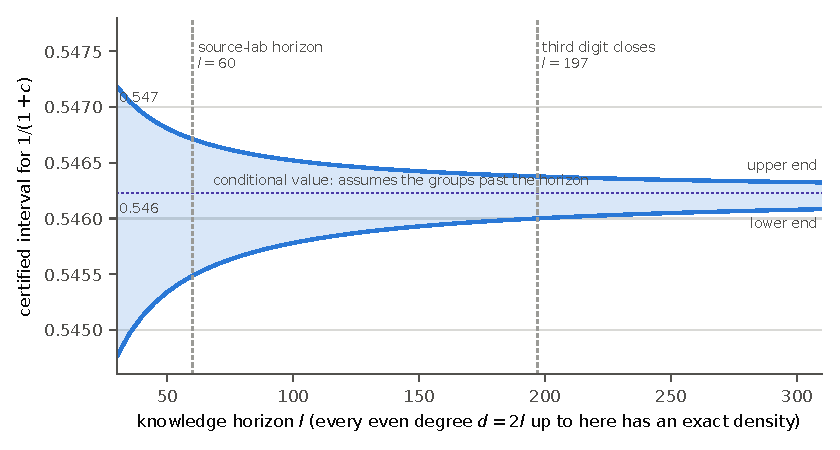
\includegraphics[width=0.64\linewidth]{fig/erdos290-liminf.pdf}
\caption{The certified interval for $1/(1+c)$ against the knowledge horizon $l$, every point re-assembled in exact rationals by the bracket module and rounded outward to twelve decimals: the band is the interval, the hairlines the decimal cells, the dotted line the conditional value of Section~\ref{sec:cond}, which assumes the groups past the horizon and is drawn in a different style for that reason. The third decimal closes at $l=\ThirdDigitL$. Data: \texttt{paper/tex/fig/erdos290-squeeze.json}.}\label{fig:liminf}
\end{figure}

\section{Both endpoints of Theorem~8, and the exact liminf}\label{sec:thm8}

Lemma~32's range $\VDCLo<c<\VDCHi$ gives $1/(1+c)\in(\VDInvLo,\VDInvHi)$ and $1/(2c)<\VDTwoCHi$; the published $\VDLo$ and $\VDHi$ are these to two decimals. Theorem~\ref{thm:bracket} with Lemmas~30 and~31 of \cite{vD24} gives
\begin{equation}\label{eq:thm8sharp}
\InvLo\;<\;\lia\;<\;\TwoCHi ,
\end{equation}
an interval of width \NewWidth{} in place of \VDWidth. The lower endpoint is fed by the upper end of $c$, which carries the unpinned tail at $\delta=1$, so it moves only as degrees are decided: $\VDLo\to\InvSixtyLo$ at the source lab's horizon and $\to\InvLo$ here. The upper endpoint $1/(2c)$ is fed by the lower end of $c$, which charges the unpinned tail zero, so no assumption about the groups past the horizon enters it; it was already $\TwoCSixtyHi$ at $L=\CitedL$, so most of the gain over $\VDHi$ is that $\VDCLo$ was a conservative floor for $c$. Both carry the Lemma~32 dependency of Table~\ref{tab:prov} and nothing else.

\paragraph{The liminf became exact.} On 31 August 2026, the day the third decimal of the bracket was posted on \cite{Issue164}, van Doorn submitted \cite{vD26}, whose Theorem~1 is $\lia=\frac1{1+c}$, with the remark that $\frac1{1+c}$ ``is approximately equal to $0.546$, although we make no effort here to calculate it as precisely as possible'', and, combining with Lemma~32, the consequence that $b(a)<a+0.55\log a$ for infinitely many $a$. The note's Section~4 states that the key step of the proof was found by a language model and that the paper is a human-written simplification of it, with the original output at \cite{GPTnote}; the proof uses no numerics, and the record here plays no role in it. Its effect on the record is that the upper endpoint of \eqref{eq:thm8sharp}, and with it the sharpening $\VDHi\to\TwoCHi$ posted the same day, is retired: not wrong, overtaken. What survives is stronger.

\begin{corollary}\label{cor:liminf}
Assuming Theorem~1 of \cite{vD26} and the Lemma~32 dependency of Table~\ref{tab:prov},
\[
\lia\in[\InvLo,\ \InvHi] .
\]
In particular $b(a)>a+\InvLoThree\log a$ for all sufficiently large $a$, and $b(a)<a+\InvHiFour\log a$ for infinitely many $a$.
\end{corollary}

To our knowledge the interval of Corollary~\ref{cor:liminf} is the sharpest stated enclosure of this liminf; the note itself states three digits as an approximation and no interval. The report page \cite{Report} has carried Theorem~1 of \cite{vD26} since early September 2026, with the two-sided reading kept as history; van Doorn acknowledged the comments on \cite{Issue164} on 8 September 2026 and pointed to the note, retiring the $1/(2c)$ endpoint. The OEIS entry he asked for in the issue is drafted in the repository and not submitted.

\section{The conditional expansion: theorem digits and expansion digits}\label{sec:cond}

Let $\mathcal A(D)$ be the assumption: for every even $d=2l\ge D$, $G_d$ is $\Sl$ or $E$, equivalently $\delta(f_d)\in[\delta_{\mathrm{hyp}}(l)-1/(2^l\,l!),\ \delta_{\mathrm{hyp}}(l)]$. It holds at every degree where the group has been decided, which by Proposition~\ref{prop:record} is every even $d\le\HorizonD$. Under $\mathcal A(D)$ the tail telescopes: $\sum_{l>N}w_l=\sum_{m=1}^{2N+1}\frac{(-1)^{m+1}}m-\log2$ exactly, and $\delta_{\mathrm{hyp}}(l)$ sits within $1/(2^{l+1}(l+1)!)$ of $1-e^{-1/2}$ by the alternating series, so the tail past a cutoff $N$ is an interval of width about $2/(2^{N+1}(N+1)!)$ times its weight, with the index-2 allowance and the alternating-series deviation carried as two separate terms.

Two enclosures of this kind are in the record. The lifted kernel, which certifies exactly only through $d=60$, assumes from $d=\CondFirstD$:
\begin{gather*}
c^*\in[\CondLo,\ \CondHi],\\
\frac1{1+c^*}=\CondInv\ldots
\end{gather*}
The first assumed degree is not asserted but read off the enclosure: its width is the sum of the carried allowances $w_l/(2^l\,l!)$ over the degrees it does not certify exactly, the largest being \CondAllowFirst{} at $l=\CondFirstL$, which caps that enclosure at \CondCap{} decimals however large the cutoff; the record publishes \CondDigits. Two checks have teeth: the enclosures at cutoffs $N=120$ and $N=200$ must intersect (the kernel's own comments record that the tail identity once shipped wrong by $8.6\times10^{-6}$ at $N=120$, an error only a cutoff-agreement check sees), and the conditional value must lie inside Theorem~\ref{thm:bracket}'s bracket. The second enclosure, \texttt{erdos290-cstar-precision.js}, moves the certified horizon to the record's, so the assumption begins at $d=\FailD$; calibrated against the lifted kernel at horizon $60$ (\PrecCalib{} digits agree) and with cutoffs $N=\PrecCutoffA$ and $\PrecCutoffB$ agreeing, it gives \CStarDigits{} decimals of each:
\begin{align*}
c^*&=0.\CStarFullA\\&\hphantom{{}=0.}\CStarFullB\ldots\\[2pt]
\frac1{1+c^*}&=0.\CZeroFullA\\&\hphantom{{}=0.}\CZeroFullB\ldots
\end{align*}
Both are written as OEIS b-files of \BfileTerms{} terms in the repository, re-generated after every horizon move and byte-identical to the live run at this build.

\paragraph{Failure semantics.} If $\mathcal A(\FailD)$ first fails at an even degree $d_0$, the density there is some value in $[0,1]$ instead of a sliver near $\DeltaLimit$, so $c^*$ moves by at most $w_{d_0/2}=1/(d_0(d_0+1))$, which is at most \FailC, and $1/(1+c^*)$ by at most $\InvDeriv$ of that (the derivative of $1/(1+x)$ at the lower end of the bracket), i.e.\ \FailInv. An entry built on the expansion would therefore be amended by raising $d_0$, never retracted. Which decimals survive is a question about decimal boundaries, not magnitudes: by interval containment, a first failure at $d_0=122$, $500$ or $1000$ preserves \SensOne, \SensTwo{} or \SensThree{} decimals of $1/(1+c^*)$ at the lifted kernel's horizon, counts it asserts at every build; a draft that reasoned from the size of the move had claimed seven at $d_0=1000$.

\paragraph{Theorem digits.} Theorem~8 of \cite{vD24} states its constants to two decimals because Lemma~32 pins $c$ to $(\VDCLo,\VDCHi)$; the third decimal of $1/(1+c)$ therefore sharpens a published theorem statement, and since \cite{vD26} it is a decimal of a constant known exactly, with no assumption about the tail behind it (the Lemma~32 group computation of Table~\ref{tab:prov} taken as given, as everywhere here). No theorem states this constant to four decimals: a fourth decimal, and the \CStarDigits{} above, sharpen a decimal expansion and nothing else. They are digits of an OEIS entry, and the drafted entry carries the assumption in its definition and the failure semantics in its comments, with the three decimals that assume nothing about the tail as the fallback an editor may prefer.

\paragraph{What a fourth digit with no tail assumption would take.} The width of Theorem~\ref{thm:bracket}'s bracket is the unpinned tail. (i) By horizon: if every further degree closes as $\mathcal A$ predicts, the fourth decimal of $1/(1+c)$ closes at $l=\FourthL$ ($d=\FourthD$), width \FourthWidth; at a cost growing as $l^{\TimeExponent}$ that is about \FourthCost{} times the cost of a degree at the present horizon, per degree. (ii) By a lemma: any proved window $\delta(f_d)\in[A,B]$ for all even $d>\HorizonD$ narrows the bracket at once, with no computation; at the present horizon the fourth decimal, the cell $[\CellLo,\CellHi)$ the conditional value sits in, needs $A>\WindowA$ and $B\le\WindowB$, and the limit $1-e^{-1/2}=\DeltaLimit$ sits inside with margins \WindowMarginLo{} below and \WindowMarginHi{} above, so a window of width $0.1$ about it would do. Two scouting observations, not in the record and not proved: with a sign kernel containing the even-weight module and a transitive $\pi(G)$, Jensen's inequality on $2^{-t}$ and Burnside's $\mathbb E[\mathrm{fix}]=1$ give $\delta\le\frac12<\WindowB$; and $\delta\ge1/r$ for a transitive group of rank $r$ \cite{DFG} would supply the floor from a rank bound. Both presuppose irreducibility of $f_d$ for large even $d$, computed in \cite{vD24} to $d\le500$ and, as far as we have seen, unproved; nothing we found concerns $\Gal(f_d)$ for large $d$.

\section{What is not claimed}\label{sec:not}

\begin{itemize}
\item Not that $G_d\cong\Sl$ for all even $d$ off the exceptional degrees, nor that $f_d$ is irreducible for all $d$ (decided through $d=\HorizonD$, resp.\ computed to $500$ in \cite{vD24}; assumed nowhere in Theorem~\ref{thm:bracket}); nor that the group drops to $E$ at every $4k(k+1)$ (Theorem~\ref{thm:law} is a containment statement; the drop is decided at the \ExcCount{} exceptional degrees $\le\ExcMaxD$).
\item Not independence from \cite{vD24} below $d=60$: the group identification there is Magma's and is taken as given; what is re-decided is irreducibility and the exceptional set.
\item Not an outside re-run: every per-degree decision, including $\delta(f_8)=25/64$, has run only on the author's machines; the request on \cite{Issue164} for an afternoon's recomputation of $\delta(f_8)$ in Sage or Magma stands. Nothing is claimed about the problem beyond the constant, and the identity of Corollary~\ref{cor:liminf} is \cite{vD26}'s.
\item Not more than three decimals with no assumption about the tail: the \CStarDigits{} decimals assume $\mathcal A(\FailD)$, and a fourth such decimal needs a lemma or a campaign, priced above.
\item Not the composition formula, which is Cullinan's \cite{Cullinan} and elementary. What is new is the characterisation of the exceptional degrees, the decided record, the certified bracket, and the grammar that makes every refusal a costed line of the record.
\end{itemize}

\cmrepro{The records: \path{certs/erdos290-tail-ext.json} (\ExtCount{} degrees, $l=\ExtFrom..\ExtTo$, written by the serial runner and the shard merge at commit \ExtGit, committed \ExtCommitDate) and the six shard files \path{certs/erdos290-tail-shard-*.json}; the lifted source-lab programs and records in \path{legacy/research/challenges/erdos290/} (the theorem checker, the pattern check, the kernel, the two Galois programs, the narrowing pipeline with its record of \NarrowGenerated, and \path{tail-deltas.json} of \LegTailGenerated), byte-pinned through \path{LIFT.json}; the bracket module \path{machine/erdos290/tail.js}; the lean fork \path{tools/galois-exceptions-lean.js} with its battery \path{tools/erdos290-lean-battery.js}; the runners \path{tools/run-erdos290-tail-ext.js} and \path{tools/run-erdos290-tail-shard.js} (\texttt{run}, then \texttt{merge}); the expansion \path{tools/erdos290-cstar-precision.js} (argument 110); the page builder \path{tools/build-report-erdos290.js}, which re-proves the theorem, reproduces the narrowing record byte for byte and re-assembles the calibrated bracket before writing \path{reports/erdos290.html} \cite{Report}. The macros of this document are written by \path{tools/paper-numbers/erdos290.js}, which re-runs the theorem checker, the kernel, the pattern check, the lean battery and the expansion, compares every recorded density to its closed form, calibrates the bracket against the $L=\CitedL$ record point and refuses when a sentence here is no longer what the record says; \path{tools/paper-numbers/erdos290-fig.py} draws the figure from that script's data. Repository commit \RepoCommit.}

{\footnotesize\begin{thebibliography}{9}
\bibitem{EG80} P.~Erd\H{o}s, R.~L.~Graham, Old and new problems and results in combinatorial number theory, Monographies de L'Enseignement Math\'ematique 28, Gen\`eve, 1980.
\bibitem{EP290} T.~F.~Bloom, Erd\H{o}s problem 290, \url{https://www.erdosproblems.com/290}, accessed 2026-10-01.
\bibitem{vD24} W.~van Doorn, On the non-monotonicity of the denominator of generalized harmonic sums, arXiv:2411.03073 (v2, 23 July 2025).
\bibitem{vD26} W.~van Doorn, The shortest harmonic sums with decreasing denominator, arXiv:2609.00104 (31 August 2026).
\bibitem{Issue164} W.~van Doorn (Woett), HELP WANTED: Computing sequence for Erd\H{o}s problem \#290, issue 164 of \texttt{teorth/erdosproblems}, opened 28 November 2025, \url{https://github.com/teorth/erdosproblems/issues/164}.
\bibitem{GPTnote} ChatGPT 5.6-Sol Pro, The sharp lower-limit constant for the first decrease of a harmonic denominator, GitHub repository \texttt{Woett/ChatGPT-s-note-on-Erdos290}, as cited in \cite{vD26}.
\bibitem{Cullinan} J.~Cullinan, The discriminant of a composition, note, Bard College, \url{https://faculty.bard.edu/cullinan/disccomp.pdf}, accessed 2026-10-01.
\bibitem{OEIS} OEIS Foundation Inc., The On-Line Encyclopedia of Integer Sequences, A033996: $8$ times triangular numbers, $a(n)=4n(n+1)$, \url{https://oeis.org/A033996}.
\bibitem{Wielandt} H.~Wielandt, Finite Permutation Groups, Academic Press, New York, 1964.
\bibitem{Cox} D.~A.~Cox, Galois Theory, 2nd ed., Wiley, 2012.
\bibitem{DFG} P.~Diaconis, J.~Fulman, R.~Guralnick, On fixed points of permutations, arXiv:0708.2643 (2007).
\bibitem{Report} C.~Toledo, Erd\H{o}s \#290: the $4k(k+1)$ theorem, cert-machine report, \url{https://www.carlostoledo.co/reports/erdos290.html}, rebuilt with every number recomputed at each build; repository \url{https://github.com/carlostoledo1891/cert-machine} (concept DOI 10.5281/zenodo.22225860), holding the records named in the reproduction section.
\end{thebibliography}}

\end{document}
